\section{An explicit cubic example and the extremal staircase}
\label{sec:example}

Take $Q=7\cdot13\cdot19=1729$. Let $\chi_7,\chi_{13},\chi_{19}$ be
the order-three characters determined by
\[
 \chi_7(3)=\zeta,\qquad\chi_{13}(2)=\zeta,
 \qquad\chi_{19}(2)=\zeta,
\]
where $3,2,2$ are primitive roots modulo $7,13,19$, respectively.
View all three as characters modulo $Q$ by the Chinese remainder theorem.
They generate a rank-three group. Consider the two products
\begin{align*}
 \mathcal L_A(s)&=
   \prod_{j=0}^{2}L(s,\chi_7^j\chi_{13})
                        L(s,\chi_7^j\chi_{13}^{-1}),\\
 \mathcal L_C(s)&=
   \prod_{j=0}^{2}L(s,\chi_7^j\chi_{19})
                        L(s,\chi_7^j\chi_{19}^{-1}).
\end{align*}
Each product has six distinct nonprincipal cubic-character factors, and
the two packets are disjoint. Their trace difference at an unramified prime
is
\[
 H(p)=
 (1+\chi_7(p)+\chi_7(p)^2)
 \bigl(\chi_{13}(p)+\chi_{13}(p)^{-1}
       -\chi_{19}(p)-\chi_{19}(p)^{-1}\bigr).
\]
It is nonzero exactly when $\chi_7(p)=1$ and exactly one of
$\chi_{13}(p),\chi_{19}(p)$ equals $1$. The three independent character
values are uniform on $\{1,\zeta,\zeta^2\}^3$. Consequently
\[
 \delta(A,C)=\frac13\frac49=\frac4{27},
 \qquad\text{agreement density}=\frac{23}{27}.
\]
Theorem~\ref{thm:cubic-min} proves that $23/27$ is the largest agreement
density possible for two distinct six-factor packets of cubic characters,
at any rank at least three. Thus the example is an optimum, rather than
just a construction with unusually large agreement.

The exact check in \code{results/cubic\_checks.json} finds 192 disagreeing
classes among the 1296 reduced residue classes modulo 1729. The first
distinguishing prime is $113$, followed by $181,197,281,293,307$.
Up to $200\,000$, 2642 of 17\,981 eligible primes disagree. That finite
frequency is illustrative; the density $4/27$ follows from the proof, not
from numerical extrapolation.

\begin{figure}[htbp]
\centering
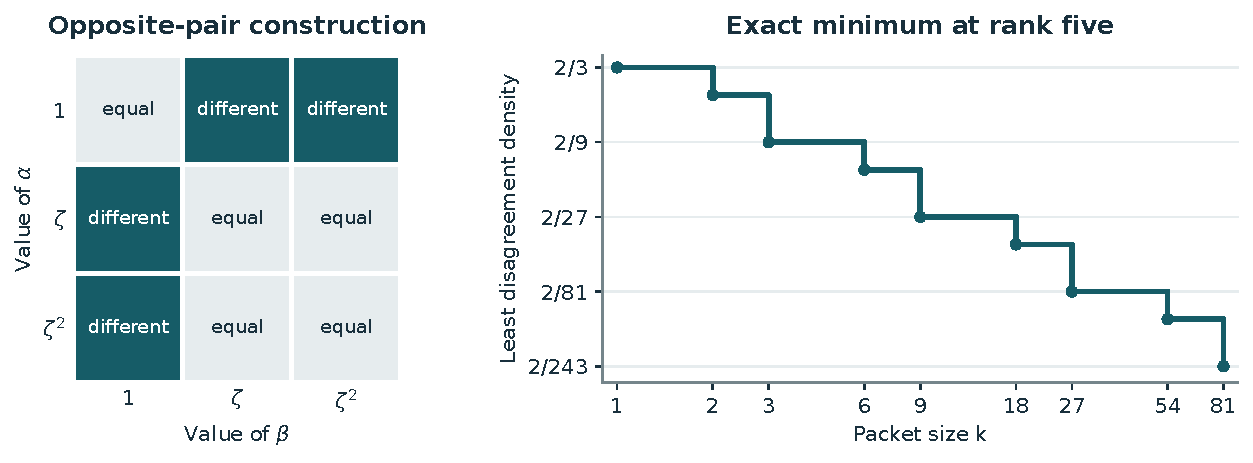
\includegraphics[width=\linewidth]{figures/cubic_staircase.pdf}
\caption{Left: the four disagreeing classes for the basic opposite-pair
construction, among nine ternary value pairs. Right: the exact minimum
disagreement as the packet size grows, at rank five; both axes are
logarithmic. The two steps per power of three reflect odd and even
Eisenstein valuations.}
\label{fig:cubic}
\end{figure}

\begin{center}
\begin{tabular}{@{}ccc@{}}
\toprule
Packet size $k$ & Least disagreement & Greatest agreement\\
\midrule
1 & $2/3$ & $1/3$\\
2 & $4/9$ & $5/9$\\
3--5 & $2/9$ & $7/9$\\
6--8 & $4/27$ & $23/27$\\
9--17 & $2/27$ & $25/27$\\
18--26 & $4/81$ & $77/81$\\
27--53 & $2/81$ & $79/81$\\
54--80 & $4/243$ & $239/243$\\
\bottomrule
\end{tabular}
\end{center}
\noindent The table holds without saturation, for example at rank $r\ge5$.
At smaller ranks, the density stops decreasing at $2/3^r$.
